\newpage
\subsection{Problem 2 - Equality Constrained Quadratic Optimization}

The second problem that this report deals with has been defined in a following way:

\begin{equation}
\begin{split}
\min_{u} \frac{1}{2} \sum_{i=1}^{n+1} (u_i - \bar{u})^2\\
s.t. \quad -u_1 + u_n = - d_0\\
u_i - u_{i+1} = 0\\
u_{n-1} - u_n - u_{n+1} = 0
\end{split}
\end{equation}
The first step we took was translation of the problem into convenient matrix notation:

\begin{equation}
\begin{split}
\min_{x} f(x) = \frac{1}{2} x'Hx + g'x\\
s.t. \quad A'x = b,
\end{split}
\end{equation}
which for $n=10$, $\bar{u} = 0.2$ and $d_0=1$ looks as follows:

\[
  H =
  \begin{bmatrix}
    1& & \\
    & \ddots & \\
    & &1
  \end{bmatrix}
\]\\

\[g=\begin{bmatrix}
	0.4 \\ . \\ . \\ . \\ 0.4
\end{bmatrix}\]\\
     
\[A=\begin{bmatrix}
	\begin{tabular}{llllllllll}
-1 & 1  & 0  & 0  & 0  & 0  & 0  & 0  & 0  & 0  \\
0  & -1 & 1  & 0  & 0  & 0  & 0  & 0  & 0  & 0  \\
0  & 0  & -1 & 1  & 0  & 0  & 0  & 0  & 0  & 0  \\
0  & 0  & 0  & -1 & 1  & 0  & 0  & 0  & 0  & 0  \\
0  & 0  & 0  & 0  & -1 & 1  & 0  & 0  & 0  & 0  \\
0  & 0  & 0  & 0  & 0  & -1 & 1  & 0  & 0  & 0  \\
0  & 0  & 0  & 0  & 0  & 0  & -1 & 1  & 0  & 0  \\
0  & 0  & 0  & 0  & 0  & 0  & 0  & -1 & 1  & 0  \\
0  & 0  & 0  & 0  & 0  & 0  & 0  & 0  & -1 & 1  \\
1  & 0  & 0  & 0  & 0  & 0  & 0  & 0  & 0  & -1 \\
0  & 0  & 0  & 0  & 0  & 0  & 0  & 0  & 0  & -1
\end{tabular}
\end{bmatrix}\]\\

\[b= \begin{bmatrix}
	\begin{tabular}{llllllllll}
-1 & 0 & 0 & 0 & 0 & 0 & 0 & 0 & 0 & 0 
\end{tabular}
\end{bmatrix}^T\]\\
The Lagrangian can then be written as a function of $n$, $\bar{u}$ and $d_0$:

\begin{equation}
L = \frac{1}{2} \sum_{i=1}^{n+1} (u_i - \bar{u})^2\\ - \sum_{i=1}^{n-2} \lambda_i(u_i-u_{i+1}) - \lambda_{n-1}(-u_1+u_n+d_0) - \lambda_{n}(u_{n-1}-u_n-u_{n+1}).
\end{equation}
or in matrix notation
\begin{equation}
L = \frac{1}{2} x'Hx + g'x - \lambda(A'x - b).\\
\end{equation}
This can be further used to form the KKT first order optimality conditions
\begin{equation}
\begin{split}
\nabla L = Hx + g - A\lambda = 0\\
s.t. \quad A'x - b = 0,
\end{split}
\end{equation}
that are necessary but in this case also sufficient for the optimality. To prove that we have to show that f(x) is a convex  function(because of minimization) and that active inequality constraints are convex. Since there are no inequality constraints (there is nothing to make them concave) and equality constraints are affine (linear) the latter requirement is met. Regarding the objective function, we can look at the coefficient by the $2^(nd)$ order term and check its sign. In our case by the highest order term $u$ we see implicit 1 which means its a convex function, therefore we have proven that KKT is necessary and sufficient for the problem at hand.

Next, we implemented multiple variations of the solvers that use different matrices factorizations, procedures but also store the matrices in dense or sparse manner. All the algorithms however output the same results being

\[
  x =
  \begin{bmatrix}
    \begin{tabular}{lllllllllll}
-0.3000 & -0.3000 & -0.3000 & -0.3000 & -0.3000 & -0.3000 & -0.3000 & -0.3000 & -0.3000 & -1.3000 & 1.0000
\end{tabular}
  \end{bmatrix}^T\]
\]
\[
  \lambda =
  \begin{bmatrix}
    \begin{tabular}{llllllllll}
-2.3000 & -2.2000 & -2.1000 & -2.0000 & -1.9000 & -1.8000 & -1.7000 & -1.6000 & -1.5000 & -1.4000
\end{tabular}
  \end{bmatrix}^T\]
\]


Once this step has been completed, we compared the performances of the solvers based on LU, LDL, Null-Space and Range-Space factorizations. For this purpose we measured the CPU time, so the time that the processing unit needed for finding the solution - that in case of multi-core processors may not be the same as the wall time - the actual time that the calculations took. By using the CPU time, we are able to objectively compare the performance of the algorithms and see how their pure implementations behave when varying the problem size. The obtained results are shown on Figure \ref{fig:all_solvers}.

\begin{figure}[ht!]
    \centering
    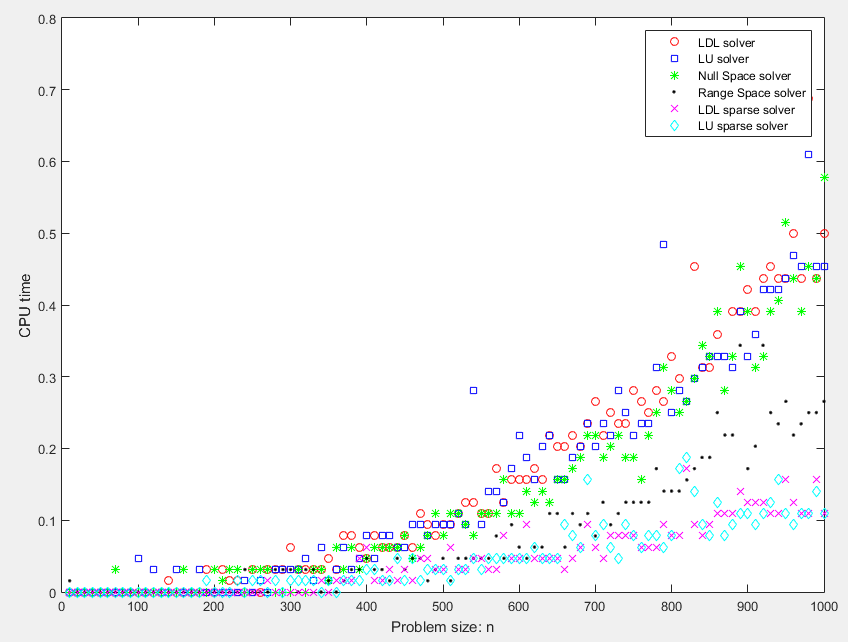
\includegraphics[width=\textwidth]{fig/all_solvers.PNG}
    \caption{Comparison of multiple QP solvers}
    \label{fig:all_solvers}
\end{figure}
From theory we would expect the LDL-based solver to be superior over LU as it requires less operations but for tested problem sizes they perform very comparably, with LDL being more stable. Interestingly, these two solvers seems to be outperformed by Null-Space solver (at least for small problem sizes) that is using QR-factorization, which is in fact slightly more computationally expensive. Further we see that Range-Space solver is a lot faster than previously presented methods, but we also know that it uses sparse structure for hessian matrix that is needed for Cholesky factorization if we want it to output 3 values in MatLab.

\begin{figure}[ht!]
    \centering
    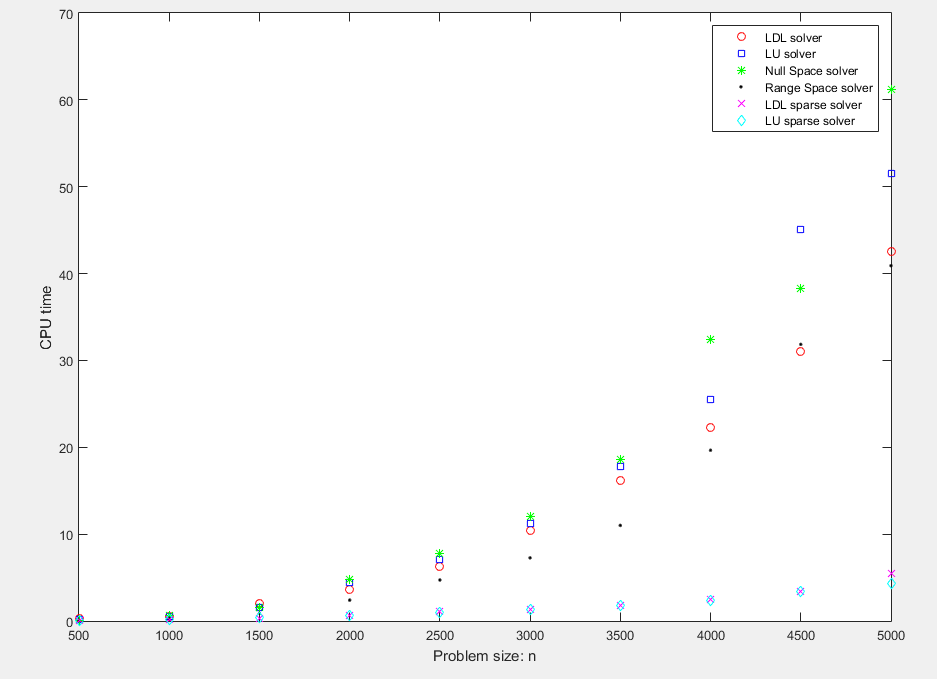
\includegraphics[width=\textwidth]{fig/bigger_prob.PNG}
    \caption{QP solvers with increased problem sizes}
    \label{fig:bigger_prob}
\end{figure}

Since the results for 3 dense solvers seemed a bit surprising, but also the problem sizes were very small, we decided to increase them up to 4000 and see if our expectations would be reflected by the times that solvers took to solve the problem. The results of this test can be seen on Figure \ref{fig:bigger_prob}. As a rule of thumb, when we want to compare the runtimes of some programs/algorithms we should either repeat the experiments multiple time and take the average or as a good practice, make sure the runtime exceeds 1s and the initialization processes are not taking the majority of the runtime. 

Based on the result of Range-Space method, we already suspect that other sparse-based solvers will outperform all above mentioned implementations as it uses less Cholesky factorization that is a bit less efficient than both LDL and LU. To support this claim we first investigated the sparsity pattern of KKT matrix and it looks as presented on Figure \ref{fig:kkt_sparsity}

\begin{figure}[ht!]
    \centering
    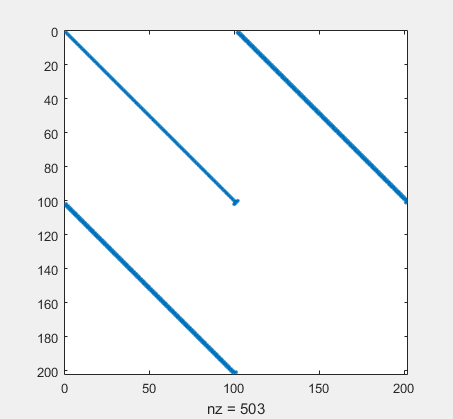
\includegraphics[width=.5\textwidth]{fig/kkt_sparsity.PNG}
    \caption{Sparsity pattern of KKT matrix}
    \label{fig:kkt_sparsity}
\end{figure}

This tells us that great majority of the KKT entires are 0's and therefore we could really take advantage of storing it as a sparse matrix. When we look at Figure \ref{fig:all_solvers} or \ref{fig:bigger_prob}, we clearly see that the variations using sparse matrices turned out to be superior. It should be also mentioned that for Range-Space solver, we make hessian (H) and matrix A sparse whereas in LDL and Lu solvers the entire KKT matrices are being converted into sparse structures and that might be the reason why there is this quite a big gap between these 3 solvers. 
\newpage